\section*{Chapter Exercises}
\addcontentsline{toc}{section}{Exercises}

\exercise{1}{chapter-crl}{Write a method that determines whether three integers are strictly increasing. Three integers $x, y,$ and $z$ are strictly increasing if $x < y < z$.}

\exercise{1}{chapter-crl}{Write conditional statements that determines if an integer $n$ is greater than $100$. If so, return the string of $n$ divided by two. If the number is less than 50, return the string of $n$ divided by five. In any other case, return the string ``N/A''.}

\exercise{1}{chapter-crl}{Given an integer variable \textit{age} in years, write conditional statements to determine if the age is able to vote in the United States. For reference, someone may legally once they turn eighteen years old.}

\exercise{1}{chapter-crl}{Write the \ttt{max} that returns the maximum of three integers $a$, $b$, and $c$. Do not use any built-in (\ttt{Math} library) methods.}

\exercise{1}{chapter-crl}{Write the \ttt{isEvenlySpaced} method, which receives three integers and returns whether they are evenly spaced. Evenly spaced means that the difference between the smallest and medium number is the same as the difference between the medium and largest number.}

\exercise{1}{chapter-crl}{In propositional logic, there are several \textit{connectives} that act on boolean truth values. These include logical conjunction $\land$, disjunction $\lor$, conditional $\to$, biconditional $\leftrightarrow$, and negation $\lnot$. We can represent \textit{schemata} as a series of composed method calls. For example, an evaluation of}

\[
    `P \to \lnot (Q \leftrightarrow \lnot R)'
\]

\noindent where `$P$' and `$R$' are assigned to \ttt{false} and `$Q$' is assigned to \ttt{true}, is equivalent to

\begin{verbatim}
public static final boolean P = false;
public static final boolean Q = true;
public static final boolean R = false;

cond(P, not(bicond(Q, not(R))))
\end{verbatim}

\noindent The presented schema resolves to \ttt{true}.

\noindent Design methods for the five connectives according to the following truth tables. These methods should be called \ttt{cond}, \ttt{bicond}, \ttt{and}, \ttt{or}, and \ttt{not}. Assume that $\top$ is \ttt{true} and $\bot$ is \ttt{false}.
\captionsetup[subfigure]{labelformat=empty}
\captionsetup[figure]{labelformat=empty}%
\begin{figure}[H]
\begin{center}
    \begin{tabular}{c|c}
         $P$&$\lnot{P}$\\
         \hline
         $\top$&$\bot$\\
         $\bot$&$\top$
    \end{tabular}
\end{center}
\caption{Truth Table of `$\lnot{P}$'}
\label{fig:ttnotp}
\end{figure}

\begin{figure}[H]
\begin{subfigure}{.5\textwidth}
\begin{center}
    \begin{tabular}{cc|c}
         $P$&$Q$&$P \land {Q} $\\
         \hline
         $\top$&$\top$&$\top$\\
         $\top$&$\bot$&$\bot$\\
         $\bot$&$\top$&$\bot$\\
         $\bot$&$\bot$&$\bot$
    \end{tabular}
\end{center}
\caption{Truth Table of `$P \land Q$'.}
\label{fig:ttpandq}
\end{subfigure}
\begin{subfigure}{.5\textwidth}
\begin{center}
    \begin{tabular}{cc|c}
         $P$&$Q$&$P\lor{Q} $\\
         \hline
         $\top$&$\top$&$\top$\\
         $\top$&$\bot$&$\top$\\
         $\bot$&$\top$&$\top$\\
         $\bot$&$\bot$&$\bot$
    \end{tabular}
\end{center}
\caption{Truth Table of `$P \lor Q$'.}
\label{fig:ttporq}
\end{subfigure}
\end{figure}

\begin{figure}[H]
\begin{subfigure}{.5\textwidth}
\begin{center}
    \begin{tabular}{cc|c}
         $P$&$Q$&$P\to{Q} $\\
         \hline
         $\top$&$\top$&$\top$\\
         $\top$&$\bot$&$\bot$\\
         $\bot$&$\top$&$\top$\\
         $\bot$&$\bot$&$\top$
    \end{tabular}
\end{center}
\caption{Truth Table of `$P \to Q$'.}
\label{fig:ttptoq}
\end{subfigure}
\begin{subfigure}{.5\textwidth}
\begin{center}
    \begin{tabular}{cc|c}
         $P$&$Q$&$P\liff{Q} $\\
         \hline
         $\top$&$\top$&$\top$\\
         $\top$&$\bot$&$\bot$\\
         $\bot$&$\top$&$\bot$\\
         $\bot$&$\bot$&$\top$
    \end{tabular}
\end{center}
\caption{Truth Table of `$P \liff Q$'.}
\label{fig:ttpiffq}
\end{subfigure}
\end{figure}

\captionsetup[subfigure]{labelformat=simple}
\captionsetup[figure]{labelformat=simple}%

\exercise{1}{chapter-crl}{Write the \ttt{isInsideCircle} method that, when given a circle centered at $(c_x, c_y)$ and radius $r$ as well as a point at $(p_x, p_y)$, returns whether the point is located strictly inside the circle.}

\exercise{1}{chapter-crl}{Write the \ttt{isInsideRectangle} method that, when given a rectangle centered at $(r_x, r_y)$, width $w$ and height $h$ as well as a point $(p_x, p_y)$, returns whether the point is located strictly inside the rectangle.}

\exercise{2}{chapter-crl}{Carlo is shipping out orders of candy to local grocery stores. Boxes have a maximum weight defined by \ttt{maxSize}, and we can (potentially) fit both small and large bars of candy in a box. Write the \ttt{fitCandy} method that, when given a number of small bars, large bars, and maximum weight, determines the number of small candy bars he can fit in the box. Large bars weigh five kilograms, and small bars weigh one kilogram. Note that Carlo always tries to fit large candies first before small. Return \ttt{-1} if it is impossible to fill the box with the given criteria. Below are some test examples. Hint: consider this as an analysis of three cases.}

\begin{verbatim}
fitCandy(4, 1, 9) -> 4
fitCandy(4, 1, 4) -> 4
fitCandy(1, 2, 6) -> 1
fitCandy(6, 1, 13) -> -1
fitCandy(60, 100, 550) -> 50
fitCandy(7, 1, 12) -> 7
fitCandy(7, 1, 13) -> -1
\end{verbatim}

\exercise{2}{chapter-crl}{An IPv4 address contains four integer values stored in four octets, separated by dots. For instance, \ttt{192.168.1.244} is a valid IPv4 address. Another example is \ttt{149.165.192.52}. Design the \ttt{isValidIpv4} method that, when given a \ttt{String}, determines whether it represents a valid IPv4 address. Each octet must be an integer between zero and 255 inclusive. Note that some IPv4 addresses are, in reality, nonsensical, e.g., \ttt{0.0.0.0}, but we will not consider these as invalid.}

\begin{verbatim}
isValidIpv4("192.168.1.244") -> true
isValidIpv4("149.165.192.52") -> true
isValidIpv4("192.168.1.256") -> false
isValidIpv4("192.168.1201.23") -> false
isValidIpv4("192.168.1201.ABC") -> false
isValidIpv4("ABC.DEF.GHI") -> false
isValidIpv4("192.168.1A6.201") -> false
\end{verbatim}

\exercise{1}{chapter-crl}{Write a method that receives a temperature as a \ttt{double} and a unit as a \ttt{char}, i.e., either \ttt{`C'} or \ttt{`F'} for Celsius and Fahrenheit respectively. Return a string representing whether the temperature is a liquid, solid, or gas at sea level.}

\exercise{1}{chapter-crl}{Write a method that translates a letter grade into a number grade. Letter grades are A, B, C, D, and F, possibly followed by + or -. Their numeric values are 4, 3, 2, 1, and 0. There is no F+ or F-. A+ increases the numeric value by 0.3, a - decreases it by 0.3. However, an A+ has value 4.0.}

\exercise{1}{chapter-crl}{Write a method that receives three strings and sorts them lexicographically. Return the sorted set of strings as a string itself, separated by commas. For example, if the input is \ttt{Charlie}, \ttt{Able}, \ttt{Baker}, you should return \ttt{Able,Baker,Charlie}.}

\exercise{1}{chapter-crl}{A year with $366$ days is called a leap year. Leap years are necessary to keep the calendar synchronized with the sun because the earth revolves around the sun once every $365.25$ days. Actually, that figure is not entirely precise, and for all dates after $1582$ the Gregorian correction applies. Usually years that are divisible by 4 are leap years, for example $1996$. However, years that are divisible by $100$ (for example, $1900$) are not leap years, but years that are divisible by $400$ are leap years (for example, $2000$). Write a method that receives a year and computes whether that year is a leap year. Use a single \ttt{if} statement and Boolean operators.}

\exercise{1}{chapter-crl}{Design the \ttt{computeDiscount(double itemCost, int age, boolean isStudent)} method that computes a discount for some item based on their age and student status according to the following criteria:}
\begin{itemize}
    \item If $\textit{age} < 18$, apply a $20\%$ discount.
    \item If $18 \leq \textit{age} \leq 25$ and they are a student, apply a $25\%$ discount. If they are not a student, do not apply a discount.
    \item If $age \geq 65$ and they are a student, apply a $30\%$ discount. If they are not a student, apply a $15\%$ discount.
    \item All other cases should not have a discount applied.
\end{itemize}
Your method should return the total cost of the item after applying the discount.

\exercise{1}{chapter-crl}{Design the \ttt{computeTaxCost(double itemCost, String state)} method that computes the tax for some item based on the state in which it is purchased. The method should return the total cost of the item, which includes the taxed amount. The tax rates are as follows:}
\begin{itemize}
    \item \ttt{"CA"}: $9.25\%$
    \item \ttt{"NY"}: $4.0\%$
    \item \ttt{"NC"}: $6.625\%$
    \item \ttt{"SC"}: $6.0\%$
    \item \ttt{"VA"}: $6.25\%$
    \item \ttt{"WA"}: $6.5\%$
    \item \ttt{"IN"}: $8.0\%$
\end{itemize}

\exercise{1}{chapter-crl}{Write the recursive method \ttt{countStr} that counts the number of times the substring \ttt{"str"} appears in a given string.}

\exercise{1}{chapter-crl}{Rewrite the \ttt{countStr} method to use tail recursion. Name this new version of the method \ttt{countStrTR}. Hint: you will need to design a \ttt{private static} helper method. The \ttt{countStrTR} method should only have one parameter.}

\exercise{1}{chapter-crl}{Write the recursive method \ttt{replaceAB} that replaces any occurrence of the character \ttt{`A'} with the character \ttt{`B'} in a given string.}

\exercise{1}{chapter-crl}{Rewrite the \ttt{replaceAB} method to use tail recursion. Name this new version of the method \ttt{replaceABTR}. Hint: you will need to design a \ttt{private static} helper method. The \ttt{replaceABTR} method should only have one parameter.}

\exercise{1}{chapter-crl}{Elephants have two ears, right? Write the recursive method \ttt{countElephantEars} that returns the total number of elephant ears that are in a group of elephants.}

\exercise{1}{chapter-crl}{Rewrite the \ttt{countElephantEars} method to use tail recursion. Name this new version of the method \ttt{countElephantEarsTR}. Hint: you will need to design a \ttt{private static} helper method. The \ttt{countElephantEarsTR} method should only have one parameter.}

\exercise{2}{chapter-crl}{This question has two parts.}
\begin{enumerate}[label=(\alph*)]
    \item Design the \ttt{isPrimeTR} tail recursive method, which receives a positive integer and determines if it is prime. Recall that a number is prime if and only if it evenly divides only one and itself. Hint: you will need to design a \ttt{private static} helper method to solve this problem.
    \item Design the \ttt{isPrimeLoop} method that solves the problem using a loop.

    If you write tests for one of these methods, you should be able to propagate it through the other, so write plenty!
\end{enumerate}

\exercise{1}{chapter-crl}{This question has two parts.}
\begin{enumerate}[label=(\alph*)]
    \item Design the \ttt{isPalindromeTR} tail recursive method, which receives a string and determines if it is a palindrome. Recall that a palindrome is a string that is the same backwards as it is forwards. E.g., ``racecar''. \textbf{Do not} use a (character) array, \ttt{StringBuilder}/\ttt{StringBuffer}, or similar, to solve this problem. It \textit{must} be naturally recursive.
    \item Design the \ttt{isPalindromeLoop} method that solves the problem using a loop. The same restrictions from the previous problem hold true for this one.

    If you write tests for one of these methods, you should be able to propagate it through the other, so write plenty!
\end{enumerate}

\exercise{1}{chapter-crl}{This question has two parts.}
\begin{enumerate}[label=(\alph*)]
    \item Design the \ttt{gcdTR} tail recursive method, which receives two integers and returns the greatest common divisor between the two. Euclid's algorithm is the basis for this approach and is a tail recursive algorithm by design.
    \item Design the \ttt{gcdLoop} method that solves the problem using a loop.

    If you write tests for one of these methods, you should be able to propagate it through the other, so write plenty!
\end{enumerate}

\exercise{1}{chapter-crl}{This question has two parts.}
\begin{enumerate}[label=(\alph*)]
    \item Design the \ttt{isNestedParenthesesTR} tail recursive method, which receives a string and determines if its parentheses pairs are ``balanced''. A pair of parentheses is balanced if it is a nesting of zero or more pairs of parenthesis, like ``(())'' or ``((()))''. Note that pairs like ``(()())'' will not be tested.

    \item Design the \ttt{isNestedParenthesesLoop} method that solves the problem using a loop.

    If you write tests for one of these methods, you should be able to propagate it through the other, so write plenty!
\end{enumerate}

\exercise{1}{chapter-crl}{This question has three parts.}
\begin{enumerate}[label=(\alph*)]
\item Design the standard recursive \ttt{collatz} method, which receives a positive integer and returns the Collatz sequence for said integer. This sequence is defined by the following recursive process:
\begin{align*}
    \ttt{collatz(1)} &= \ttt{1}\\
    \ttt{collatz(n)} &= \ttt{collatz(3 * n + 1)} \text{ if \ttt{n} is odd.}\\
    \ttt{collatz(n)} &= \ttt{collatz(n / 2)} \text{ if \ttt{n} is even.}
\end{align*}
The sequence generated is the numbers received by the method until the sequence reaches one (note that it is an open research question as to whether this sequence converges to one for every positive integer). So, \ttt{collatz(5)} returns the following \ttt{String} of comma-separated integers: \ttt{"5,16,8,4,2,1"}. \textbf{The last number cannot have a comma afterwards}.

\item Then, design the \ttt{collatzTR} method that uses tail recursion and accumulators to solve the problem. Hint: you will need to design a \ttt{private static} helper method to solve this problem.

\item Finally, design the \ttt{collatzLoop} method that solves the problem using a loop.

If you write tests for one of these methods, you should be able to propagate it through the rest, so write plenty!
\end{enumerate}

\exercise{1}{chapter-crl}{This question has three parts.}
\begin{enumerate}[label=(\alph*)]
\item Design the standard recursive \ttt{parenthesesDepth} method, which receives a string of parentheses and returns an integer representing the ``depth'' at the end of the string. Each instance of \texttt{(} increments the depth counter, and each instance of \texttt{)} decrements the depth counter. So, e.g., \texttt{"((())()))))(()"} is $1+1+1-1-1+1-1-1-1-1-1+1+1=-2$.

\item Then, design the \ttt{parenthesesDepthTR} method that uses tail recursion and accumulators to solve the problem. Hint: you will need to design a \ttt{private static} helper method to solve this problem.

\item Finally, design the \ttt{parenthesesDepthLoop} method that solves the problem using a loop.

If you write tests for one of these methods, you should be able to propagate it through the rest, so write plenty!
\end{enumerate}

\exercise{1}{chapter-crl}{This question has three parts.}
\begin{enumerate}[label=(\alph*)]
\item Design the standard recursive \ttt{countdown} method, which receives an \texttt{int} $n \geq 0$ and returns a \texttt{String} containing a sequence of the even numbers from $n$ down to $0$ inclusive, separated by commas.

\item Then, design the \ttt{countdownTR} method that uses tail recursion and accumulators to solve the problem. Hint: you will need to design a \ttt{private static} helper method to solve this problem.

\item Finally, design the \ttt{countdownLoop} method that solves the problem using a loop.

If you write tests for one of these methods, you should be able to propagate it through the rest, so write plenty!
\end{enumerate}

\exercise{2}{chapter-crl}{Design the static \ttt{indexOf} method, which receives two \ttt{String}s \ttt{s}, \ttt{key}, and returns the first index of \ttt{key} in \ttt{s}. Note that \ttt{key} may be any arbitrary string and not just a a single character. If \ttt{key} is not in \ttt{s}, return \ttt{-1}.}

\exercise{2}{chapter-crl}{Design the static \ttt{substring} method, which receives a \ttt{String} and two integers \ttt{low}, \ttt{high}, and returns the substring between these indices. If either are out of bounds of the string, return \ttt{null}.}

\exercise{1}{chapter-crl}{Design the static \ttt{isEqualTo} method, which receives two strings $s_1$ and $s_2$, and determines whether they are lexicographically equal. You cannot use the built-in \ttt{equals} or \ttt{compareTo} methods.}

\exercise{2}{chapter-crl}{Design the static \ttt{compareTo} method, which receives two \ttt{String}s \ttt{s1}, \ttt{s2}, and compares their contents lexicographically. If \ttt{s1} is less than \ttt{s2}, return \ttt{-1}. If \ttt{s1} is greater than \ttt{s2}, return \ttt{1}. Otherwise, return \ttt{0}. Note that our implementation of \ttt{compareTo} will differ from Java's in that, if \ttt{s1} has less characters than \ttt{s2}, we return \ttt{-1}; if \ttt{s2} has less characters than \ttt{s1}, we return \ttt{1}. Otherwise, we do the character-by-character comparison.}

\exercise{2}{chapter-crl}{Design the \ttt{trim} method, which receives a \ttt{String} \ttt{s} and a character \ttt{ch}, and returns a string with all leading and trailing occurrences of \ttt{ch} removed. For instance, \ttt{trim("aaHelloa", \textquotesingle{}a\textquotesingle)} returns \ttt{"Hello"}. Hint: while you cannot use Java's \ttt{substring} method, you can certainly use the one you wrote previously to solve this problem!}

\exercise{1}{chapter-crl}{Design the \ttt{trimSpace} method, which receives a \ttt{String} \ttt{s} and returns a new string with all leading and trailing spaces removed.}

\exercise{1}{chapter-crl}{Design the \ttt{containsMiddleABC} method, which receives a \ttt{String} $s$ and returns whether $s$ contains the substring \ttt{"ABC"} in the ``middle''. We define the ``middle'' as the point where number of characters on the left and right differ by at most one. \textbf{You cannot use any \ttt{String} methods to solve this problem except \ttt{.length} and \ttt{.charAt}}.}
    \begin{verbatim}
assertTrue(middleABC("helloABChiya!"));
assertTrue(middleABC("ABC"));
assertTrue(middleABC("aABCc!"));
assertFalse(middleABC("notInTheMiddleABCmid!"));
    \end{verbatim}

\exercise{1}{chapter-crl}{Design the \ttt{censor} method, which receives a String $s$ and another String $c$. It should return a ``censored'' version of $s$, wherein each instance of $c$ in $s$ is replaced by asterisks. \textbf{You cannot use any \ttt{String} methods to solve this problem except \ttt{.length} and \ttt{.charAt}}.}

\exercise{1}{chapter-crl}{Design the \ttt{isSelfDividing} method, which receives an integer $n$ and returns whether the sum of its digits evenly divide $n$. You must perform the arithmetic manually; you cannot convert the value to a \ttt{String} or use an array. }

\exercise{1}{chapter-crl}{Design the \ttt{allSelfDividing} method, which receives an integer $n$ and returns whether each digit evenly divides $n$. If any digit is zero, then return \ttt{false}. You must perform the arithmetic manually; you cannot convert the value to a \ttt{String} or use an array.}

\exercise{1}{chapter-crl}{Design the \ttt{strSumNums} that computes the sum of each \textit{positive integer} ($\geq 0$) in a \ttt{String} $s$. See the below test cases for examples. You may assume that each integer in $s$, should there be any, is in the bounds of a positive \ttt{int}, i.e., $0$ and $2^{31}-1$. Hint: use \ttt{Character.isDigit} to test whether a character $c$ is a digit, and \ttt{Integer.parseInt} to convert a \ttt{String} to an \ttt{int}.}
\begin{verbatim}
assertEquals(100, strSumNums("hello50how20are30you?"));
assertEquals(10, strSumNums("t1h1i1s1i1s1e1a1s1y1!"));
assertEquals(0, strSumNums("there are no numbers :(")));
assertEquals(0, strSumNums("still 0 just 0 zero0!"));
assertEquals(500000, strSumNums("500000"));
\end{verbatim}

\exercise{2}{chapter-crl}{Design the \ttt{stripComments} method that, when given a \ttt{String} containing a (valid) Java program, returns a string where all comments (single-line, multi-line, and Java documentation) have been removed. You cannot use any \ttt{String} helper methods (e.g., \ttt{strip}, \ttt{split}) to solve this problem nor can you use regular expressions.}

\exercise{1}{chapter-crl}{Write a method that approximates $\pi$ using the following formula:}
\[
    \pi = 4 \cdot \left(1 - \frac{1}{3} + \frac{1}{5} - \frac{1}{7} + \frac{1}{9} - \frac{1}{11} + \frac{1}{13} - \frac{1}{15} + \frac{1}{17} - \cdots \right)
\]
That is, given an input number $n$, compute that many terms of the above sequence. Return the difference between this approximation and Java's built-in \ttt{Math.PI} using \ttt{Math.abs}.

\exercise{1}{chapter-crl}{Write a method that converts a positive integer into a \ttt{String} that represents its binary counterpart. We present some examples below.}

\begin{verbatim}
toBinary(13) => 1101
toBinary(144) => 10010000
toBinary(25) => 11001
\end{verbatim}

\exercise{1}{chapter-crl}{Write a method that, when given a string, looks for a mirror image (backwards) string at both the beginning and end of the
given string. In other words, zero or more characters at the very beginning of the given string, and at the very end of the string in reverse order (possibly overlapping). For example, the string \ttt{"abXYZba"} has the mirror end \ttt{"ab"}.}

\begin{verbatim}
mirrorEnds("abXYZba") => ab
mirrorEnds("abca")    => a
mirrorEnds("aba")     => aba
\end{verbatim}

\exercise{2}{chapter-crl}{Write the \ttt{multTable} method that, when given two integers $a$ and $b$ such that $a < b$, computes the ``multiplication table'' from $a$ to $b$. We provide some test cases below. Note that the newline is just for formatting purposes.}
\begin{verbatim}
multTable(3, 3) => "1*1=1,1*2=2,1*3=3,2*1=2,2*2=4,
                    2*3=6,3*1=3,3*2=6,3*3=9"
multTable(2, 6) => "1*1=1,1*2=2,1*3=3,1*4=4,1*5=5,
                    1*6=6,2*1=2,2*2=4,2*3=6,2*4=8,
                    2*5=10,2*6=12"
\end{verbatim}

\exercise{3}{chapter-crl}{The \textit{definite integral} of a function $f$, defined as $\int_{a}^{b} f(x)\;\text{d}x$, produces the area under the curve of $f$ on the interval $[a, b]$. The thing is, though, integrals are defined in terms of \textit{Riemann summations}, which provide estimations on the area under a curve.} Riemann sums approximate the area by creating rectangles of a fixed width $\Delta$, as shown in ~\ref{fig:riemannf} for an arbitrary function $f$. Left-Riemann, right-Riemann, and midpoint-Riemann approximations define the focal point, i.e., the height, of the rectangle. Notice that, in Figure ~\ref{fig:riemannf}, we use a midpoint-Riemann sum with $\Delta = 0.2$, in which the collective sum of all the rectangle areas is the Riemann approximation. Your job is to use this idea to approximate the area of a circle.

\begin{figure}[H]
\begin{center}
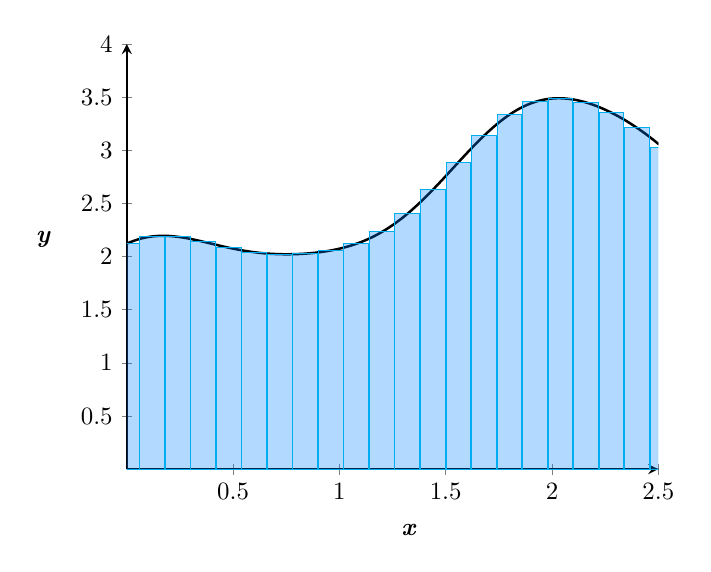
\begin{tikzpicture}[scale=0.9,
    declare function={
    % f(\x)=(\x^2)+9*\x+7;
        f(\x)=2+cos(deg(\x-2))+cos(deg(3*\x))/2+sin(cos(5*\x))/8 + cos(deg(7*\x))/28;
    }
]
\begin{axis}[
    axis lines = middle,
    xtick ={0.5, 1.0, 1.5, 2.0, 2.5, 3.0, 3.5},
    ytick ={0, 0.5, 1, 1.5, 2.0, 2.5, 3, 3.5, 4, 4.5, 5, 5.5},
    % xticklabels = {$a=x_0$,$x_1$,$x_2$,$x_3$, $\ldots$, $x_{n-1}$,$x_n=b$},
    ymin = 0,
    ymax = 4,
    xmin = 0,
    xmax = 2.5,
    x=3cm,y=1.5cm,
    axis line style = thick,
    xlabel style={at={(.5,0)},above right,yshift=-30pt},
    ylabel style={at={(0,.5)},above right,xshift=-40pt},
    xlabel={$\textit{\textbf{x}}$},
    ylabel={$\textit{\textbf{y}}$},
    % extra x ticks={1.3,1.85,2.2,2.7,3.2,3.75}
]

\addplot [
    % domain=1:4,
    samples=300,
    % line width=1pt,
    % fill=red, draw=none,
    % fill opacity=0.1
] {f(x)} \closedcycle;

\addplot [
    domain=0:5,
    samples=300,
    line width = 1pt, black] {f(x)};

\addplot[ybar, bar width=10pt, domain=1:4,samples at={0, 0.12, 0.24, 0.36, 0.48, 0.60, 0.72, 0.84, 0.96, 1.08, 1.20, 1.32, 1.44, 1.56, 1.68, 1.80, 1.92, 2.04, 2.16, 2.28, 2.40, 2.52, 2.64, 2.76, 2.88, 3.00, 3.12, 3.24, 3.36, 3.48}, fill=blue!50!cyan,fill opacity=0.3, draw=cyan]
  {f(x)};
\end{axis}
\end{tikzpicture}
\end{center}
\caption{Midpoint-Riemann Approximation of a Function}
\label{fig:riemannf}
\end{figure}

Design the \ttt{circleArea} method, which receives a radius $r$ and a delta $\Delta$. It computes (and returns) a left/right-Riemann approximation of the area of a circle. Hint: if you compute the left/right-Riemann approximation of one quadrant, you can very easily obtain an approximation of the total circle area. We illustrate this hint in Figure ~\ref{fig:circlearea} where $\Delta=0.5$ and its radius $r=2$. Note that the approximated area will vary based on the chosen Riemann approximation.\footnote{A left-Riemann sum under-approximates the area, whereas a right-Riemann sum provides an over-approximation. A midpoint approximation uses the average between the left and right approximations. It should be noted that, in the general case, these statements do not hold as they depend on the interval we integrate our function over.} Further note that no calculus knowledge is necessary to solve this exercise.

\begin{figure}[H]
\begin{center}
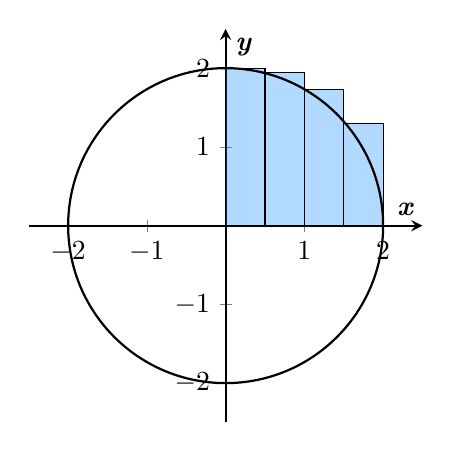
\begin{tikzpicture}
\begin{axis}[
    axis lines = middle,
    xtick ={-3,-2,-1,0,1,2,3},
    ytick ={-3,-2,-1,0,1,2,3},
    % xticklabels = {$a=x_0$,$x_1$,$x_2$,$x_3$, $\ldots$, $x_{n-1}$,$x_n=b$},
    ymin = -2.5,
    ymax = 2.5,
    xmin = -2.5,
    xmax = 2.5,
    x=1cm,y=1cm,
    axis line style = thick,
    xlabel={$\textit{\textbf{x}}$},
    ylabel={$\textit{\textbf{y}}$},
    % extra x ticks={1.3,1.85,2.2,2.7,3.2,3.75}
]
\end{axis}

  \draw[fill=blue!50!cyan,fill opacity=0.3] (2.5,2.5) rectangle (3,4.5);
  \draw[fill=blue!50!cyan,fill opacity=0.3] (3.0,2.5) rectangle (3.5,4.44);
  \draw[fill=blue!50!cyan,fill opacity=0.3] (3.5,2.5) rectangle (4.0,4.23);
  \draw[fill=blue!50!cyan,fill opacity=0.3] (4,2.5) rectangle (4.5,3.80);
\draw[thick] (2.5,2.5) circle (2);
\end{tikzpicture}

\end{center}
\caption{Right-Riemann Approximation of a Function}
\label{fig:circlearea}
\end{figure}